\documentclass[10pt,a4paper]{article}
\usepackage[utf8]{inputenc}
\usepackage[spanish]{babel}
\usepackage{amsmath}
\usepackage{amsfonts}
\usepackage{amssymb}
\usepackage[T1]{fontenc} 
\usepackage[left=2.00cm, right=2.00cm, top=2.00cm, bottom=2.00cm]{geometry}
\usepackage{acronym}
\usepackage{listings}
\usepackage{graphicx}
\graphicspath{ {images/} }
\usepackage{hyperref}

\usepackage{multirow}
\usepackage[table,xcdraw]{xcolor}

\usepackage[export]{adjustbox}
\usepackage{subcaption}

\usepackage[ruled]{algorithm2e}

%%Sobre el código
\usepackage{xcolor}
\usepackage{xparse}
\NewDocumentCommand{\codeword}{v}{%
	\texttt{\textcolor{blue}{#1}}%
}

\setlength{\parindent}{1em}
\setlength{\parskip}{1em}




\title{
Práctica 2\\
\large Aprendizaje Automático \\
}

\author{
Alejandro Palencia Blanco\\
}

\date{01/05/2021}



\begin{document}

\maketitle

\newpage

\tableofcontents

\newpage

\section{Ejercicio sobre la complejidad de H y el ruido}

El objetivo de este ejercicio será aprender la dificultad que introduce en un problema de aprendizaje la aparición de ruido. Esto supone, a su vez, que la elección de una clase de funciones adecuada para resolverlo resulte más complicada.

\subsection{Simulación de nubes de puntos con distribución uniforme y gaussiana}

En este primer apartado, simularemos dos nubes de puntos de tamaño $N=50$. Una de ellas la generaremos a partir de una distribución uniforme sobre el cuadrado $[-50,50] \times [-50,50]$, mientras que en la otra usaremos una distribución gaussiana con media 0 y varianzas 5 y 7 para las coordenadas x e y, respectivamente. En la figura \ref{fig:ej1.1_nubes} podemos ver las nubes de puntos obtenidas.

\begin{figure}[h]
	\begin{subfigure}{0.5\textwidth}
		\centering
		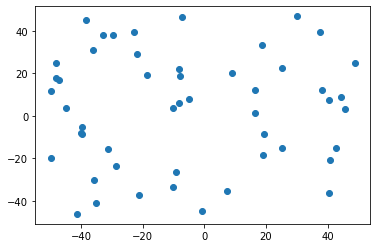
\includegraphics[width=\textwidth]{ej1.1_nube_unif}
		\caption{Nube de puntos uniforme}
	\end{subfigure}
	\begin{subfigure}{0.5\textwidth}
		\centering
		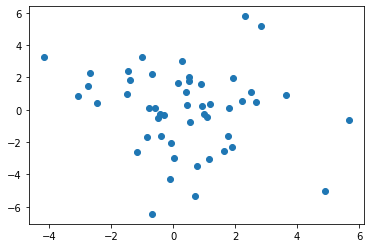
\includegraphics[width=\textwidth]{ej1.1_nube_gauss}
		\caption{Nube de puntos gaussiana}
	\end{subfigure}
	\caption{Nubes de puntos obtenidas mediante distribuciones uniforme y gaussiana}
	\label{fig:ej1.1_nubes}
\end{figure}




\subsection{Valoración de la influencia del ruido según la clase de funciones}

Ahora, valoraremos cómo influye el ruido según la complejidad de la clase de funciones que seleccionemos. De nuevo, tomamos otra muestra uniforme en el cuadrado $[-50,50] \times [-50,50]$, pero esta vez de tamaño $N=100$. Además, simulamos una recta $y=ax+b$ que pase por dicha región, la cual a su vez nos permite etiquetar a los puntos de la muestra tomada según queden por encima o por debajo de ella. Es decir, un punto $(x,y)$ de la muestra recibirá la etiqueta $signo(y-ax-b) \in \{-1,1\}$. En la figura \ref{fig:ej1.2_nube_etiq} podemos ver la nube etiquetada a partir de la recta.

\begin{figure}[h]
	\centering
	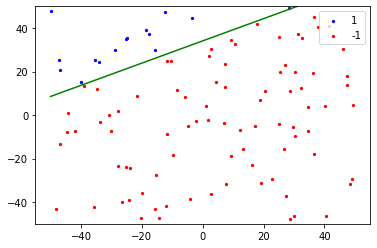
\includegraphics[width=0.5\textwidth]{ej1.2_nube_etiq}
	\caption{Nube de puntos uniforme etiquetada a partir de la recta}
	\label{fig:ej1.2_nube_etiq}
\end{figure}

Observamos, como es esperable, que todos los puntos están bien etiquetados con respecto a la recta.

A continuación, añadimos un 10\% de ruido en cada una de las clases; es decir, modificamos aleatoriamente las etiquetas del 10\% de los datos con etiqueta positiva, y procedemos de forma análoga para los que tienen etiqueta negativa. Por tanto, ahora los puntos que han sufrido un cambio en su etiqueta estarán mal clasificados con respecto a la recta. La figura \ref{fig:ej1.2_nube_ruido} muestra la nube de puntos después de introducir ruido.

\begin{figure}[h]
	\centering
	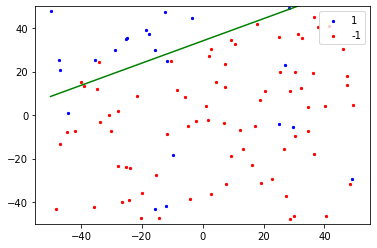
\includegraphics[width=0.5\textwidth]{ej1.2_nube_ruido}
	\caption{Nube de puntos uniforme etiquetada con un 10\% de ruido}
	\label{fig:ej1.2_nube_ruido}
\end{figure}

Por último, tomaremos cuatro funciones que igualadas a cero definen curvas cónicas que usaremos como frontera de clasificación. Estas funciones son:

\begin{itemize}
	\item $f_1(x,y) = (x-10)^2 + (y-20)^2 - 400$
	\item $f_2(x,y) = 0.5(x+10)^2 + (y-20)^2 - 400$
	\item $f_3(x,y) = 0.5(x-10)^2 - (y+20)^2 - 400$
	\item $f_4(x,y) = y - 20x^2 - 5x + 3$
\end{itemize}

El resultado de visualizarlas sobre la nube de puntos anterior podemos verlo en la figura \ref{fig:ej1.2_nubes_conicas}. Los errores de clasificación sobre la muestra (porcentaje de puntos mal clasificados) obtenidos por cada una de ellas son:

\begin{itemize}
	\item $f_1$ (circunferencia): 72\%
	\item $f_2$ (elipse): 78\%
	\item $f_3$ (hipérbola): 29\%
	\item $f_4$ (parábola): 15\%
\end{itemize}

Se puede apreciar que los errores de clasificación de la circunferencia y la elipse, 72\% y 78\% respectivamente, son demasiado altos, incluso superiores al 50\%. Esto significa que, con un método que clasificase los puntos de forma aleatoria obtendríamos, en promedio, mejores resultados que usando alguna de estas dos funciones. 

Por otro lado, la hipérbola y la parábola obtienen errores mucho más bajos, del 29\% y 15\% respectivamente. Sin embargo, esto no se debe a la complejidad de las mismas, sino a las peculiaridades de la muestra generada. Si analizamos únicamente la muestra etiquetada, podemos ver que aproximademante el 85\% de los puntos tienen la etiqueta -1 (son rojos) mientras que el 15\% restante tienen la etiqueta 1 (son azules). Ahora, mirando las regiones de clasificación de la hipérbola y la parábola, vemos que ambas tienen una región negativa (roja) mucho más amplia que la positiva (azul), lo cual explica que los errores de clasificación sean mucho menores.

Es especialmente llamativo el caso de la parábola, pues si analizamos su región positiva podemos apreciar que ningún punto cae dentro de ella, luego en esencia está clasificando todos los puntos con la etiqueta -1. Por tanto, estamos usando una función relativamente compleja como es la parábola para realizar una clasificación tan simple como es aquella que asigna a todos los puntos la misma etiqueta.

Si comparamos estos resultados con los obtenidos por la recta usada para etiquetar los puntos, vemos que ninguna de las cuatro curvas cónicas ni siquiera consigue igualar el error de clasificación obtenido por la recta (que sabemos que se encuentra en torno al 10\% después de añadir ruido).

Después de este análisis, podemos llegar a las siguientes conclusiones:

\begin{itemize}
	\item Una mayor complejidad en la clase de funciones no asegura que los errores de clasificación vayan a ser menores. Por tanto, es posible que haya funciones más complejas que realicen una peor clasificación que otras más simples.
	\item Las cuatro funciones de este apartado han sido seleccionadas sin llevar a cabo ningún proceso de aprendizaje sobre los datos de la muestra. Por tanto, es esperable que obtengan malos resultados en términos de clasificación, y en caso de obtener buenos resultados, que éstos sean debidos a cuestiones puramente fortuitas. Esto pone de manifiesto la importancia del proceso de aprendizaje para resolver un problema de esta naturaleza.
	\item Como en un problema real es inevitable que el proceso de extracción de datos introduzca en ellos una determinada cantidad de ruido, es fundamental tener en cuenta cómo afecta este ruido al proceso de aprendizaje. En el ejemplo que acabamos de desarrollar, vemos que incluso la recta que hemos usado para etiquetar los puntos clasifica de forma errónea un 10\% de los mismos, que son precisamente aquellos que se han visto afectados por el ruido. Es importante destacar que obtendríamos este mismo porcentaje de error si repitiésemos el experimento cambiando la función usada para etiquetar por otra. Por tanto, obtener un determinado porcentaje de error debido al ruido es algo inevitable.
\end{itemize}

\begin{figure}[h]
	\begin{subfigure}{0.5\textwidth}
		\centering
		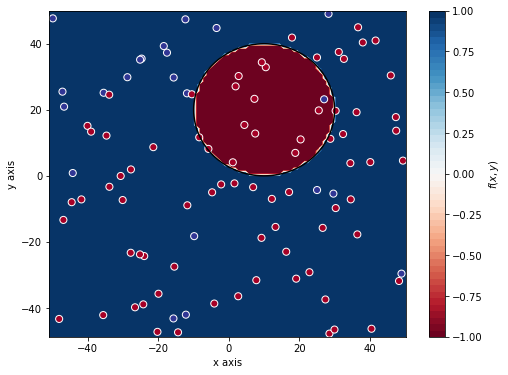
\includegraphics[width=\textwidth]{ej1.2_nube_f1}
		\caption{Función $f_1$ (circunferencia)}
	\end{subfigure}
	\begin{subfigure}{0.5\textwidth}
		\centering
		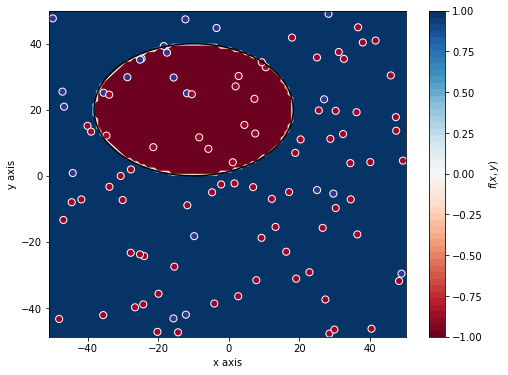
\includegraphics[width=\textwidth]{ej1.2_nube_f2}
		\caption{Función $f_2$ (elipse)}
	\end{subfigure}
	\begin{subfigure}{0.5\textwidth}
		\centering
		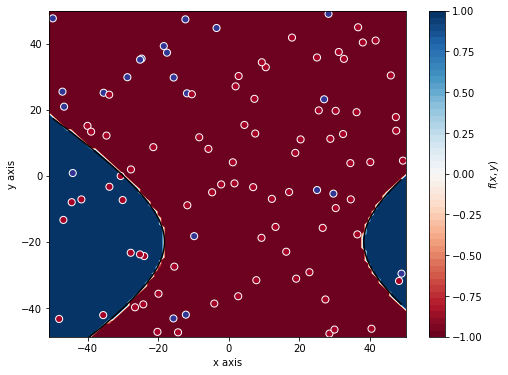
\includegraphics[width=\textwidth]{ej1.2_nube_f3}
		\caption{Función $f_3$ (hipérbola)}
	\end{subfigure}
	\begin{subfigure}{0.5\textwidth}
		\centering
		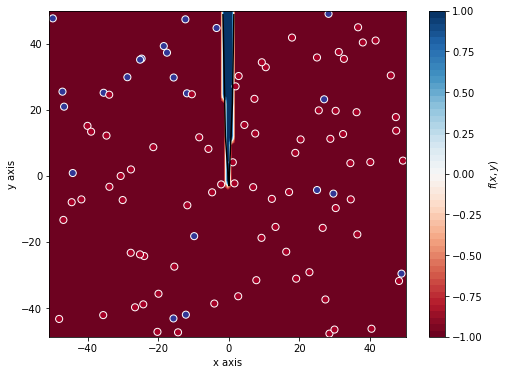
\includegraphics[width=\textwidth]{ej1.2_nube_f4}
		\caption{Función $f_4$ (parábola)}
	\end{subfigure}
	\caption{Cónicas usadas como frontera de clasificación sobre la nube de puntos}
	\label{fig:ej1.2_nubes_conicas}
\end{figure}



\newpage

\section{Modelos lineales}

En este ejercicio, haremos uso de dos modelos lineales alternativos a la Regresión Lineal vista en la práctica anterior.

\subsection{Algoritmo Perceptrón}

El primer modelo lineal que usaremos será aquel que tiene al Perceptrón como algoritmo de aprendizaje. Este es un modelo de clasificación lineal que calcula el hiperplano solución a un problema de clasificación binaria, representado a través de un vector $w$ de pesos (los coeficientes del hiperplano). El algoritmo Perceptrón recibe como parámetros la matriz que representa los items de la muestra, el vector de etiquetas, el número máximo de iteraciones permitidas y el valor inicial del vector de pesos.

\subsubsection{Ejecución sobre los datos sin ruido simulados en el ejercicio anterior}

En este apartado, ejecutaremos el algoritmo Perceptrón sobre la muestra sin ruido del ejercicio anterior con distintos valores para el vector de pesos inicial. Concretamente, inicializaremos primero el algoritmo con el vector cero, y luego realizaremos otras 10 ejecuciones inicializándolo con vectores aleatorios en el intervalo $[0,1]$. El número máximo de iteraciones lo fijaremos a 100000 en todas las ejecuciones. 

Después de realizar todas las ejecuciones, obtenemos que el número de iteraciones necesarias para converger en el caso del vector cero es 2500, mientras que para los vectores aleatorios en $[0,1]$ se necesitan en promedio 25020 iteraciones. En todas las ejecuciones, el número de iteraciones necesarias es inferior al número máximo de iteraciones fijado, lo cual implica que siempre se llega a una recta que es capaz de clasificar los puntos sin cometer ningún error. Esto era algo esperable, pues los datos han sido previamente etiquetados con una recta, luego la muestra es linealmente separable y el Perceptrón, bajo estas condiciones, siempre es capaz de llegar a una solución óptima en un número de iteraciones finito.

Por otro lado, apreciamos que el número de iteraciones necesarias para el vector cero es 10 veces menor que el promedio de iteraciones necesarias para los vectores aleatorios en $[0,1]$. Por tanto, este hecho parece indicar que tomar un vector inicial cero es la forma más inteligente de inicializar el algoritmo para conseguir una convergencia más rápida.



\subsubsection{Ejecución sobre los datos con ruido simulados en el ejercicio anterior}

Ahora realizaremos el mismo experimento de antes, pero usaremos la muestra del ejercicio anterior sobre la que se introdujo un 10\% de ruido. Obtenemos que, en todas las ejecuciones, el número de iteraciones realizadas coincide con el número máximo de iteraciones fijado, 100000. Este comportamiento diferente se debe precisamente al ruido introducido en la muestra, pues hace que ésta pase a ser no linealmente separable. Por tanto, el algoritmo Perceptrón es incapaz de encontrar una solución, ya que no existe ningún hiperplano que obtenga un error dentro de la muestra igual a 0.

Como alternativa a Perceptrón para resolver un problema en el que tenemos una muestra no linealmente separable, podemos usar el algoritmo Pocket. Este es una variante de Perceptrón que siempre guarda la mejor solución encontrada hasta el momento.



\subsection{Regresión Logística}

El segundo modelo lineal que usaremos es Regresión Logística. Este modelo tiene a Gradiente Descendente Estocástico como algoritmo de aprendizaje y calcula una función que devuelve la probabilidad de que un item pertenezca a la clase con etiqueta 1. En nuestro caso, calcularemos una función ligeramente diferente, la cual devolverá para un item el valor 1 si la probabilidad de que ese item pertenezca a la clase 1 es mayor o igual a 0.5, y devolverá 0 en caso contrario.

\subsubsection{Experimento}

El experimento consistirá en generar dos muestras, una de entrenamiento y otra de test, y aplicar Regresión Logística sobre la de entrenamiento. Posteriormente, se calculará tanto el número de épocas que tarda el algoritmo en converger como los errores de entropía cruzada y de clasificación (porcentaje de items mal clasificados) para ambas muestras. La muestra de entrenamiento tendrá tamaño $N=100$, se generará aleatoriamente mediante una distribución uniforme sobre el cuadrado $[0,2] \times [0.2]$ y será etiquetada tomando como frontera de decisión una recta, también generada aleatoriamente. La muestra de test será generada de forma análoga y etiquetada usando la misma recta, pero tendrá tamaño 1000.

Este experimento será repetido 100 veces y se obtendrán los valores promedio de las épocas invertidas y de los errores mencionados anteriormente.

En cuanto al algoritmo SGD, éste recibirá como parámetros los items de la muestra, las etiquetas de dichos items, el vector de pesos inicial (que será el vector cero), la tasa de aprendizaje (fijada a 0.01), el error que marca el criterio de parada (fijado a 0.01), el tamaño de minibatch (fijado a 1) y el número máximo de épocas (fijado a 10000). El algoritmo parará cuando se haya llegado al número máximo de épocas fijado o cuando la distancia (norma euclídea) entre los pesos de la iteración actual y la iteración anterior sea menor que el error fijado. Considero importante destacar que he probado con varios tamaños de minibatch (concretamente 1, 4 y 10) y aquel que obtiene los errores más bajos es 1.



\subsubsection{Resultados}

Después de ejecutar el experimento 100 veces, se han obtenido los siguientes resultados promedios:

\begin{itemize}
	\item Error de entropía cruzada para la muestra de entrenamiento: 0.0833
	\item Error de entropía cruzada para la muestra de test: 0.09
	\item Error de clasificación para la muestra de entrenamiento: 0.013
	\item Error de clasificación para la muestra de test: 0.0196
	\item Número de épocas necesarias para converger: 322.12
\end{itemize}

En un primer vistazo, los errores de clasificación nos permiten hacernos una idea de la calidad de la solución obtenida. Vemos que estos errores se encuentran entre el 1 y el 2\%, luego parece que la solución obtenida es razonablemente buena.

Por otro lado, teniendo en cuenta que se ha usado la misma recta como frontera de decisión para etiquetar los puntos de ambas muestras, es esperable que los puntos mal clasificados se encuentren muy cercanos a esta recta. Si a esto le sumamos el hecho de que, cuanto mayor sea el tamaño de la muestra de test, mayor será la probabilidad de encontrar más puntos cercanos a la frontera, podría ocurrir que los errores en test aumentasen de forma considerable si la solución obtenida no fuese lo suficientemente buena. Sin embargo, podemos comprobar que, a pesar de que la muestra de test sea 10 veces más grande que la de entrenamiento, los errores en ambas son muy parecidos; lo cual parece indicar que la solución calculada sí que se comporta de forma adecuada fuera de la muestra de entrenamiento.



\newpage

\section{Bonus}

\subsection{Planteamiento del problema de clasificación binaria}

En este ejercicio, consideramos el conjunto de los dígitos manuscritos 4 y 8. Partimos de una muestra de entrenamiento y otra de test con 1194 y 366 elementos, respectivamente. Sobre ellos se han medido dos características: intensidad promedio y simetría. Podemos ver las muestras etiquetadas en la figura \ref{fig:bonus_muestras}.

\begin{figure}[h]
	\begin{subfigure}{0.5\textwidth}
		\centering
		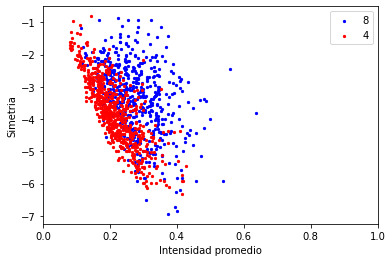
\includegraphics[width=\textwidth]{bonus_train}
		\caption{Entrenamiento}
	\end{subfigure}
	\begin{subfigure}{0.5\textwidth}
		\centering
		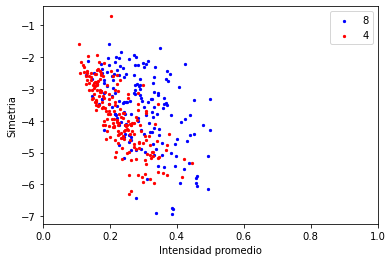
\includegraphics[width=\textwidth]{bonus_test}
		\caption{Test}
	\end{subfigure}
	\caption{Muestras de entrenamiento y test}
	\label{fig:bonus_muestras}
\end{figure}

Sobre estos datos, aplicaremos los siguientes modelos lineales:

\begin{itemize}
	\item Regresión Lineal con el algoritmo Gradiente Descendente Estocástico (SGD)
	\item Clasificación Lineal con el algoritmo PLA-Pocket
	\item Regresión Lineal con SGD junto con PLA-Pocket, usando los pesos obtenidos por el primero como los pesos iniciales del segundo
\end{itemize}



\subsection{Aplicación de Regresión Lineal y PLA-Pocket}

Empezamos ejecutando SGD en el modelo de Regresión Lineal. Empezamos con todos los pesos iniciales a cero, fijamos una tasa de aprendizaje de 0.01, un error de 0.001 para el criterio de parada, un tamaño de minibatch de 50 y un número máximo de 1000 épocas. A continuación, ejecutamos PLA-Pocket, también con los pesos iniciales a cero y con un número máximo de 10000 iteraciones. Por último, ejecutamos PLA-Pocket pasándole como pesos iniciales aquellos obtenidos en la ejecución de SGD y con un número máximo de 1000 iteraciones.

En la figura \ref{fig:bonus_funciones_estimadas} podemos ver las funciones estimadas por cada modelo sobre ambas muestras. A simple vista, parece que las 3 rectas estimadas son muy parecidas y separan razonablemente bien ambas muestras.

\begin{figure}
	\begin{subfigure}{0.5\textwidth}
		\centering
		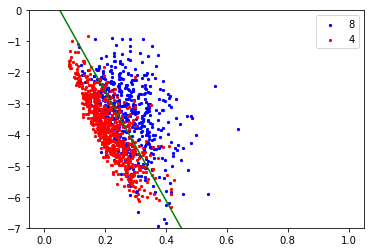
\includegraphics[width=\textwidth]{bonus_reglin_train}
		\caption{Regresión Lineal (entrenamiento)}
	\end{subfigure}
	\begin{subfigure}{0.5\textwidth}
		\centering
		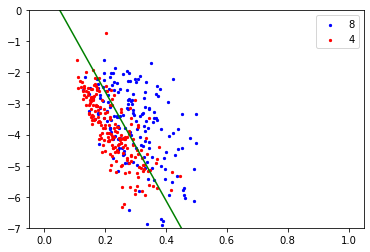
\includegraphics[width=\textwidth]{bonus_reglin_test}
		\caption{Regresión Lineal (test)}
	\end{subfigure}
	\begin{subfigure}{0.5\textwidth}
		\centering
		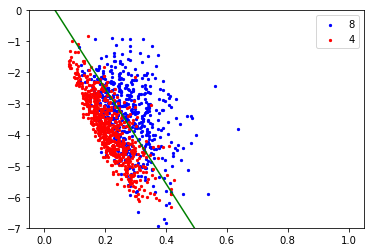
\includegraphics[width=\textwidth]{bonus_pocket_train}
		\caption{PLA-Pocket (entrenamiento)}
	\end{subfigure}
	\begin{subfigure}{0.5\textwidth}
		\centering
		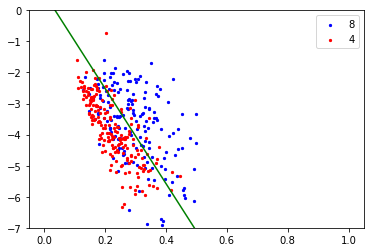
\includegraphics[width=\textwidth]{bonus_pocket_test}
		\caption{PLA-Pocket (test)}
	\end{subfigure}
	\begin{subfigure}{0.5\textwidth}
		\centering
		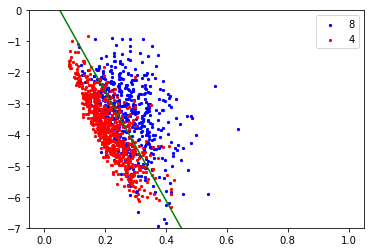
\includegraphics[width=\textwidth]{bonus_rl_p_train}
		\caption{Reg. Lin. + PLA-Pocket (entrenamiento)}
	\end{subfigure}
	\begin{subfigure}{0.5\textwidth}
		\centering
		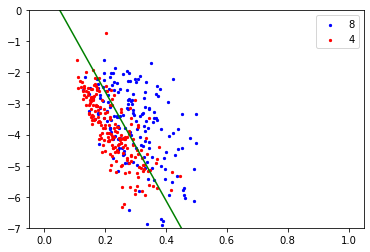
\includegraphics[width=\textwidth]{bonus_rl_p_test}
		\caption{Reg. Lin. + PLA-Pocket (test)}
	\end{subfigure}
	\caption{Funciones estimadas por los distintos métodos lineales sobre las muestras de entrenamiento y de test}
	\label{fig:bonus_funciones_estimadas}
\end{figure}

Los errores obtenidos para cada modelo se muestran en el cuadro \ref{fig:bonus_errores}. Podemos observar que los errores de clasificación obtenidos por todos ellos son muy parecidos, aumentando ligeramente entre un 2 y un 3\% de entrenamiento a test. La función estimada en Regresión Lineal también experimenta este ligero aumento de entrenamiento a test en su error cuadrático medio.

También se puede ver que, tanto las funciones estimadas como los errores de clasificación obtenidos en Regresión Lineal y en Reg. Lin. + PLA-Pocket son idénticos. Esto nos informa de que la ejecución de PLA-Pocket sobre los pesos devueltos por SGD no consigue llegar en ninguna iteración a unos pesos que reduzcan el error de los pesos iniciales, luego acaba devolviendo los mismos pesos iniciales que se le pasaron.

\begin{table}
	\centering
	\begin{tabular}{l|r|c|c|}
		\cline{2-4}
		\multicolumn{1}{c|}{\textbf{}}                                                                          & \multicolumn{1}{c|}{\textbf{Regresión Lineal}} & \textbf{PLA-Pocket}                      & \textbf{Reg. Lin. + PLA-Pocket}          \\ \hline
		\multicolumn{1}{|l|}{\begin{tabular}[c]{@{}l@{}}Error Cuadrático Medio \\ (entrenamiento)\end{tabular}} & 0.6470                             & -                                        & -                                        \\ \hline
		\multicolumn{1}{|l|}{\begin{tabular}[c]{@{}l@{}}Error Cuadrático Medio \\ (test)\end{tabular}}          & 0.7061                             & -                                        & -                                        \\ \hline
		\multicolumn{1}{|l|}{\begin{tabular}[c]{@{}l@{}}Error de Clasificación \\ (entrenamiento)\end{tabular}} & 0.2253                            & \multicolumn{1}{r|}{0.2320}  & \multicolumn{1}{r|}{0.2253} \\ \hline
		\multicolumn{1}{|l|}{\begin{tabular}[c]{@{}l@{}}Error de Clasificación \\ (test)\end{tabular}}          & 0.2432                            & \multicolumn{1}{r|}{0.2623} & \multicolumn{1}{r|}{0.2432} \\ \hline
	\end{tabular}
	\caption{Errores obtenidos para cada modelo}
	\label{fig:bonus_errores}
\end{table}

Por último, calculamos cotas de error para los verdaderos valores de $E_{out}$. En todos ellos fijaremos una tolerancia $\delta = 0.05$, luego la probabilidad de que las cotas que calculemos se cumplan será de $1-\delta = 0.95$ al menos. Para $E_{in}$, aplicaremos la expresión que usa la cota de generalización de Vapnik-Chervonenkis, teniendo en cuenta que en todos los modelos, la dimensión de VC de la clase de funciones que usan es 3:

$$E_{out} \leq E_{in} + \sqrt{\frac{8}{N}\log{\frac{4((2N)^{d_{VC}}+1)}{\delta}}}$$



Para $E_{test}$, usaremos la cota basada en la desigualdad de Hoeffding. Como en el momento de obtener esta cota ya hemos fijado nuestra función hipótesis, aplicaremos la expresión en la que $|H| = 1$:

$$E_{out} \leq E_{test} + \sqrt{\frac{1}{2N}\log{\frac{2}{\delta}}}$$

Las cotas basadas en $E_{in}$ son las siguientes:

\begin{itemize}
	\item Regresión Lineal: $E_{out} \leq 0.6470 + 0.4309 = 1.0779$
	\item PLA-Pocket: $E_{out} \leq 0.2320 + 0.4309 = 0.6629$
	\item Reg. Lin + PLA-Pocket: $E_{out} \leq 0.2253 + 0.4309 = 0.6562$
\end{itemize}

Las cotas basadas en $E_{test}$ son las siguientes:

\begin{itemize}
\item Regresión Lineal: $E_{out} \leq 0.7061 + 0.0710 = 0.7771$
\item PLA-Pocket: $E_{out} \leq 0.2623 + 0.0710 = 0.3333$
\item Reg. Lin + PLA-Pocket: $E_{out} \leq 0.2432 + 0.0710 = 0.3142$
\end{itemize}

Observamos que las cotas basadas en $E_{test}$ son en los tres métodos mejores que las basadas en $E_{in}$, a pesar de que hemos visto anteriormente que los errores de test son ligeramente mayores que los de entrenamiento. Esto se debe a que el segundo sumando de la cota siempre es mucho más bajo en las cotas basadas en $E_{test}$ que en las de $E_{in}$, lo cual a su vez está provocado, bajo mi punto de vista, por las siguientes razones:

\begin{itemize}
	\item El tamaño de la muestra juega un papel fundamental, pues cuanto mayor sea, menor será la cota que obtengamos. En $E_{in}$, el segundo sumando es $\mathcal{O} \left( \sqrt{d_{VC}\frac{\log{N}}{N}} \right)$, mientras que en $E_{test}$ tenemos que es $\mathcal{O} \left( \sqrt{\frac{1}{N}} \right)$. Por tanto, aunque la muestra de entrenamiento sea 3 veces más grande que la de test, la función $\frac{1}{N}$ decrece más rápidamente que $\frac{\log{N}}{N}$, lo cual juega a favor de la cota basada en $E_{test}$.
	\item Aunque la dimensión de Vapnik-Chervonenkis mejore en gran medida la cota basada en $E_{in}$ al no depender del cardinal de $H$, en este aspecto es peor que la cota basada en $E_{test}$, pues ésta última no depende ni de $d_{VC}$ ni de $|H|$.
	\item Las constantes involucradas en ambas expresiones también pueden tener un impacto considerable. Se puede ver que en la cota basada en $E_{in}$, estas constantes se encuentran en los numeradores, lo cual contribuye a empeorar el valor de la cota obtenida; mientras que en $E_{test}$ una de estas constantes se encuentra en un denominador.
\end{itemize}






\end{document}



